% Báo cáo ACL — đánh giá lại CIRAG trên ViMQA
% Biên dịch: pdflatex main -> bibtex main -> pdflatex main -> pdflatex main
% Hình trong report/figures/ sinh tự động bằng scripts/make_figures.py

\documentclass[11pt]{article}
\usepackage{acl}
\usepackage{times}
\usepackage{latexsym}
\usepackage[T5,T1]{fontenc}
\usepackage[utf8]{inputenc}
\usepackage{microtype}
\usepackage{graphicx}
\usepackage{booktabs}
\usepackage{amsmath}
\usepackage{amssymb}
\usepackage{multirow}
\usepackage[vietnamese]{babel}
\usepackage{tikz}
\usetikzlibrary{arrows.meta, positioning, fit, backgrounds}

% Nới ngưỡng xếp hình để hình nằm gần phần thảo luận tương ứng.
% \paragraph mặc định chèn 3.25ex phía trên, quá rộng cho tiêu đề chạy dòng.
\makeatletter
\renewcommand\paragraph{\@startsection{paragraph}{4}{\z@}%
  {1.2ex \@plus1ex \@minus.2ex}{-1em}{\normalfont\normalsize\bfseries}}
\makeatother

\setcounter{topnumber}{2}
\renewcommand{\topfraction}{0.9}
\renewcommand{\textfraction}{0.07}
\renewcommand{\floatpagefraction}{0.75}

\title{Đánh giá lại CIRAG trên Hỏi đáp Đa bước tiếng Việt:\\
       điều kiện dừng theo câu từ chối và một phép kiểm thay thế trên bằng chứng}

\author{
  Tan Nguyen Dang Duy, Huy Tran Anh, Tien Le Van, and Tram Nguyen Hong \\
  \textit{Faculty of Information Technology} \\
  \textit{University of Science, VNU-HCM} \\
  Ho Chi Minh City, Vietnam \\
  \texttt{\{25C1502208, 25C1100780, 25C1106995, 25C1107056\}@student.hcmus.edu.vn}
}

\begin{document}
\maketitle

\begin{abstract}
CIRAG \citep{wei2026cirag} nén các đoạn văn đã truy hồi thành triple $(s,r,o)$ để bớt nhiễu,
và các tác giả báo cáo mức cải thiện lớn so với những phương pháp truy hồi lặp trước đó.
Chúng tôi cài đặt lại phương pháp này, rồi chạy thử trên chính bộ dữ liệu và mô hình nền mà
bài báo gốc dùng. Bản cài đặt tái lập được khoảng cách họ công bố trong phạm vi 0,6 điểm EM.
Nhưng khi chúng tôi chuyển sang ViMQA \citep{le2022vimqa}, bộ hỏi đáp đa bước tiếng Việt,
khoảng cách đó biến mất. Bốn thí nghiệm có kiểm soát cho thấy nguyên nhân không nằm ở bản
cài đặt, prompt tiếng Việt, một khâu trong pipeline chạy sai hay năng lực mô hình nền. Nguyên
nhân nằm ở điều kiện dừng của phương pháp. ACMG chỉ mở rộng ngữ cảnh khi mô hình tự nói ra
rằng nó không trả lời được, nghĩa là nó tin vào phán đoán của mô hình thay vì tự kiểm tra
ngữ cảnh. Mô
hình nền càng mạnh thì càng ít khi nói vậy, nên hệ thống hầu như luôn dừng ở mức ngữ cảnh
hẹp nhất và trả lời sai từ đó. Chúng tôi
thay điều kiện đó bằng một phép kiểm đặt trên chính bằng chứng. Phép kiểm này đòi tập triple
lõi phải đến từ đủ số tài liệu mà câu hỏi đa bước cần, và nó nâng EM từ 50,80 lên 60,40
mà không tốn thêm lời gọi mô hình nào.
\end{abstract}

\section{Giới thiệu}
\label{sec:intro}

Sinh có tăng cường truy hồi \citep{lewis2020rag} hoạt động tốt với câu hỏi đơn giản nhưng
gặp khó ở suy luận đa bước, vì truy hồi một lượt không gom được các bằng chứng liên kết với
nhau. Truy hồi lặp \citep{trivedi2023ircot} giảm bớt khó khăn này bằng cách chia thành nhiều
lượt, mỗi lượt dùng thông tin vừa thu được để tạo truy vấn tiếp theo. Gần đây, một số công
trình thay đoạn văn bằng triple làm đơn vị truy hồi \citep{fang2024trace, fang2025kirag}
nhằm thu hẹp phạm vi bằng chứng và giảm nhiễu.

CIRAG \citep{wei2026cirag} nhắm vào hai vấn đề riêng biệt của hướng truy hồi lặp trên
triple. Vấn đề thứ nhất là mở rộng tham lam theo một đường. Các phương pháp trước chỉ giữ một
triple tốt nhất ở mỗi bước, nên sai sót ở bước đầu lan sang các bước sau, đồng thời những
nhánh bằng chứng song song cần cho câu hỏi phức tạp bị bỏ qua. Vấn đề thứ hai nằm ở
mức ngữ cảnh: triple có cấu trúc rõ và ít nhiễu nhưng thiếu ngữ cảnh, còn đoạn văn đủ ngữ
cảnh nhưng nhiều nhiễu, nên không có mức cố định nào phục vụ được mọi câu hỏi.

Nhằm hạn chế mở rộng tham lam, CIRAG đề xuất module truy hồi ICI (Iterative
Construction-Integration), xây dựng trên mô hình Kiến tạo và Tích hợp trong tâm lý học nhận
thức \citep{kintsch1978ci}. Giai đoạn kiến tạo gom triple của các đoạn vừa truy hồi thành
một tập ứng viên rộng, giai đoạn tích hợp để mô hình nền chọn ra tập triple lõi thực sự cần
cho câu hỏi rồi sinh truy vấn kế tiếp. Vì được phép chọn nhiều triple cùng lúc, tập lõi có
thể chứa bằng chứng của nhiều nhánh suy luận khác nhau thay vì chỉ một nhánh.

Nhằm khớp mức ngữ cảnh với nhu cầu của câu hỏi, CIRAG đề xuất module sinh ACMG (Adaptive
Cascaded Multi-Granularity Knowledge-Enhanced Generation). Ở mỗi mức, hệ thống đưa cho mô
hình phần ngữ cảnh của mức đó và yêu cầu trả lời, kèm chỉ dẫn rằng nếu ngữ cảnh chưa đủ thì
phải trả về một câu từ chối định sẵn thay vì đoán. Chính câu từ chối đó là tín hiệu để mở
rộng ngữ cảnh. Module bắt đầu ở mức triple, và chỉ chuyển sang mức câu rồi mức đoạn văn khi
nhận được câu từ chối.

Chúng tôi cài đặt lại CIRAG và đánh giá trên ViMQA \citep{le2022vimqa}, bộ hỏi đáp đa bước
tiếng Việt. Bản cài đặt tái lập được lợi thế mà bài báo gốc công bố khi chạy trên chính bộ
dữ liệu của họ, nhưng lợi thế đó không xuất hiện trên ViMQA, và phần còn lại của báo cáo đi
tìm lý do. Đóng góp gồm bốn điểm:

\begin{itemize}
  \itemsep0.1em
  \item Chúng tôi kiểm chứng bản cài đặt trên 2WikiMultihopQA với đúng mô hình nền mà bài
        báo gốc dùng. Khoảng cách giữa CIRAG và IRCoT đo được chỉ lệch 0,6 điểm EM so với
        con số họ công bố (\S\ref{sec:results}).
  \item CIRAG dựa vào câu từ chối của mô hình để biết ngữ cảnh đã đủ hay chưa. Dấu hiệu này
        sai theo cả hai chiều: mô hình từ chối cả khi bằng chứng đã có sẵn, và trả lời cả
        khi bằng chứng còn thiếu (\S\ref{sec:analysis}).
  \item Chúng tôi thay dấu hiệu đó bằng một phép kiểm trên chính bằng chứng. Câu hỏi đa bước
        cần dữ kiện từ ít nhất hai tài liệu, nên hệ thống chỉ dừng khi tập triple lõi đã
        đến từ đủ hai tài liệu. Phép kiểm nâng EM từ 50,80 lên 60,40 mà không tốn thêm
        lời gọi mô hình nào (\S\ref{sec:fix}).
  \item Chúng tôi loại trừ bốn cách giải thích khác cho việc lợi thế của CIRAG không xuất
        hiện trên ViMQA: lỗi cài đặt, prompt tiếng Việt, một khâu trong pipeline chạy sai, và
        năng lực mô hình nền (\S\ref{sec:backbone}).
\end{itemize}

\section{Công trình liên quan}
\label{sec:related}

\paragraph{Truy hồi lặp trên văn bản.} IRCoT \citep{trivedi2023ircot} xen kẽ sinh chuỗi suy
luận với truy hồi, dùng câu suy luận vừa sinh làm truy vấn kế tiếp. Self-Ask
\citep{press2023selfask} phân rã câu hỏi thành các câu hỏi con tường minh. Vì mỗi lượt
đưa thêm nguyên đoạn văn vào ngữ cảnh, nhiễu tích tụ dần qua các vòng.

\paragraph{Truy hồi lặp trên triple.} Để giảm nhiễu đó, một nhánh nghiên cứu đổi đơn vị truy
hồi từ đoạn văn sang triple. HippoRAG \citep{jimenez2024hipporag} dựng đồ thị tri thức từ
triple trích được, còn KiRAG \citep{fang2025kirag} nối dần các triple thành một chuỗi bằng
chứng qua từng vòng lặp. Đổi lại, chúng chỉ giữ một triple tốt nhất ở mỗi bước và cố định
biểu diễn ở mức triple.

CIRAG khác hai nhánh trên ở đúng hai điểm đó. Nó giữ một tập triple lõi thay vì một chuỗi
đơn, và mở rộng ngữ cảnh theo bậc thay vì cố định ở một mức.

\section{Phương pháp}
\label{sec:cirag}

CIRAG chạy hai module nối tiếp (Hình~\ref{fig:pipeline}): ICI truy hồi và lọc bằng chứng
thành một tập triple lõi, còn ACMG sinh câu trả lời từ tập đó. Bài báo gốc còn một module
thứ ba, Trajectory Distillation, huấn luyện một mô hình nhỏ bắt chước quỹ đạo suy luận của
mô hình lớn để giảm chi phí. Chúng tôi không cài module này, nên mọi con số trong báo cáo
đối chiếu với cấu hình \emph{w/o TD} của bài báo gốc.

\begin{figure*}[t]
\centering
\begin{tikzpicture}[
  font=\small,
  b/.style={draw, rounded corners=2pt, align=center, inner sep=4pt, minimum height=7mm},
  lv/.style={b, fill=blue!7, minimum width=20mm},
  ar/.style={-{Latex[length=1.8mm]}, gray!80, line width=0.6pt},
  lb/.style={font=\footnotesize, inner sep=1.5pt},
]
% ── ICI: vòng lặp giữa hai giai đoạn ──
\node[b, minimum width=24mm]                       (q)    {truy vấn $q_t$};
\node[b, right=11mm of q, minimum width=30mm]      (cand) {top-$N$ triple ứng viên};
\node[b, right=11mm of cand, minimum width=26mm, fill=orange!15] (f) {tập triple lõi $F$};

\draw[ar] (q)    -- node[lb, above] {kiến tạo} (cand);
\draw[ar] (cand) -- node[lb, above] {tích hợp} (f);
\draw[ar] (f.north) -- ++(0,4mm) -| node[lb, pos=0.25, above] {$q_{t+1}$, lặp tối đa $L$ vòng} (q.north);

% ── ACMG: cascade nối tiếp, mở rộng ngữ cảnh khi bị từ chối ──
\node[lv, below=13mm of q]    (t)  {triple $F$};
\node[lv, right=11mm of t]    (se) {câu $S$};
\node[lv, right=11mm of se]   (d)  {đoạn $D$};

\draw[ar] (t)  -- node[lb, above] {từ chối} (se);
\draw[ar] (se) -- node[lb, above] {từ chối} (d);

% F sinh ra cả ba mức
\draw[ar, dashed] (f.south) -- ++(0,-6.5mm) -| (t.north);
\draw[ar, dashed] (f.south) -- ++(0,-6.5mm) -| (se.north);
\draw[ar, dashed] (f.south) -- ++(0,-6.5mm) -| (d.north);
\node[lb, right=2mm of d, align=left] {đáp án lấy ở mức\\đầu tiên không từ chối};
\node[lb, left=2mm of t, align=right] {ACMG};
\end{tikzpicture}
\caption{Quy trình CIRAG. ICI lặp giữa giai đoạn kiến tạo và giai đoạn tích hợp để thu tập
triple lõi $F$. ACMG thử sinh câu trả lời trên $F$ trước, chỉ leo sang mức câu rồi mức đoạn
khi mô hình trả về câu từ chối. Mũi tên nét đứt cho thấy cả ba mức đều suy ra từ $F$, nên
thiếu sót của giai đoạn tích hợp lan sang cả ba (\S\ref{sec:limit-empty}).}
\label{fig:pipeline}
\end{figure*}

\paragraph{ICI.} Mỗi vòng lặp gồm hai giai đoạn. Giai đoạn kiến tạo truy hồi top-$K$ đoạn
cho truy vấn $q_t$, gom triple của các đoạn đó rồi xếp hạng lấy top-$N$ ứng viên. Giai
đoạn tích hợp giao tập ứng viên cùng lịch sử $H_{<t}$ cho mô hình nền, để mô hình giữ lại
tập triple lõi $F_t$ và sinh truy vấn $q_{t+1}$. Vòng lặp dừng khi mô hình sinh
\texttt{<no question>}, tối đa $L$ vòng.

Mỗi triple đều lưu vết câu và đoạn đã sinh ra nó. Hai ánh xạ ngược này, ký hiệu $M^S$ và
$M^D$, cho phép từ $F$ dựng ra tập câu $S = M^S(F)$ và tập đoạn $D = M^D(F)$. Ba tập $F$,
$S$, $D$ chính là ba mức ngữ cảnh mà ACMG sử dụng.

\paragraph{ACMG.} Hệ thống lần lượt đưa $F$, rồi $S$, rồi $D$ cho mô hình và yêu cầu trả
lời. Nếu ngữ cảnh chưa đủ, mô hình phải trả về một câu từ chối định sẵn. Đáp án được lấy ở
mức đầu tiên mà mô hình không từ chối:
\begin{equation}
\label{eq:acmg}
g^\star = \min_{\prec}\{g \in G : \mathrm{Suf}(a^{(g)}) = 1\},\quad a^\star = a^{(g^\star)}
\end{equation}
trong đó $\mathrm{Suf}(a)$ nhận giá trị đúng khi $a$ không thuộc mẫu từ chối. Nếu không có
mức nào thoả, hệ thống lùi về câu trả lời mức tài liệu. Hai chi tiết ở đây quyết định phần
sau của báo cáo: $\mathrm{Suf}$ chỉ quan sát câu trả lời chứ không quan sát ngữ cảnh, và cả
ba mức đều dựng từ một tập $F$ duy nhất. \S\ref{sec:analysis} cho thấy mỗi chi tiết dẫn tới
một kiểu lỗi riêng.

\section{Dữ liệu}
\label{sec:data}

ViMQA \citep{le2022vimqa} là bộ hỏi đáp đa bước tiếng Việt do người viết ra từ các bài
Wikipedia tiếng Việt, tổ chức theo cấu trúc HotpotQA \citep{yang2018hotpotqa}. Mỗi câu hỏi
kèm mười đoạn văn, trong đó hai đoạn chứa bằng chứng và tám đoạn gây nhiễu.

Chúng tôi lấy ngẫu nhiên 500 câu hỏi từ tập validation. Nếu mỗi câu hỏi chỉ tìm trong mười
đoạn đi kèm nó thì hệ thống gần như luôn
lấy đúng cả hai đoạn bằng chứng, và khâu truy hồi mất ý nghĩa. Theo cách làm của IRCoT,
chúng tôi hợp nhất đoạn của mọi câu hỏi rồi khử trùng lặp theo tiêu đề, thu được một kho
ngữ liệu dùng chung gồm 1.969 đoạn.

\section{Thiết lập thực nghiệm}
\label{sec:setup}

Siêu tham số giữ nguyên theo bài báo gốc ($K{=}10$, $N{=}30$, $L{=}4$). Chúng tôi thay hai
thành phần cho phù hợp với tiếng Việt. Thứ nhất, embedding dùng Vietnamese\_Embedding, đạt
recall@10 bằng 0,920 trên kho 1.969 đoạn. Thứ hai, prompt trích triple viết lại bằng tiếng
Việt, trích được 22.697 triple cho toàn kho. Mô hình suy luận là Gemini 2.5 Flash, còn khâu
trích triple dùng bản Flash Lite.

\paragraph{Độ đo.} Gọi $\hat{a}$ là câu trả lời của hệ thống, $a$ là đáp án tham chiếu và
$\nu(\cdot)$ là hàm chuẩn hoá. EM bằng $1$ khi $\nu(\hat{a})$ và $\nu(a)$ là hai chuỗi giống hệt nhau, còn F1 là trung
bình điều hoà của độ chính xác và độ phủ tính trên số token dùng chung. F1 không xét token
nằm ở đâu, còn EM đòi đúng cả thứ tự.

Tiếng Việt buộc chúng tôi điều chỉnh $\nu$ ở hai điểm. Thứ nhất, cùng một chữ có dấu có thể
lưu bằng hai chuỗi byte khác nhau mà hiển thị giống hệt nhau, nên $\nu$ quy mọi chuỗi về một
dạng Unicode chuẩn trước khi so. Thứ hai, một từ tiếng Việt có thể gồm nhiều âm tiết
(``học sinh'' là một từ nhưng hai âm tiết), và F1 thay đổi theo cách tách nên chúng tôi báo
cáo cả hai.

\paragraph{Kiểm định ý nghĩa thống kê.} Hai phương pháp trả lời cùng một tập câu hỏi, nên
phần lớn câu chúng cùng đúng hoặc cùng sai. Chỉ những câu một bên đúng còn bên kia sai mới
phân biệt được hai phương pháp, và kiểm định McNemar chỉ đếm nhóm câu đó: nếu hai phương
pháp ngang nhau thì số câu nghiêng về mỗi bên phải xấp xỉ bằng nhau. Giá trị $p$ nhỏ nghĩa
là chênh lệch quan sát được khó xảy ra do may rủi.

\paragraph{EM phạt cả câu trả lời đúng nội dung.} EM chỉ cho điểm khi hai chuỗi giống hệt
nhau, nên mọi chênh lệch độ dài giữa câu trả lời và đáp án tham chiếu đều thành điểm 0.
Chênh lệch này xảy ra theo hai chiều. Chiều thứ nhất là đáp án tham chiếu dài: hệ thống nêu
đủ các thành phần nhưng đảo thứ tự, cho F1 bằng 1,00 mà EM bằng 0, và trong 99 câu có đáp án
dài hơn năm âm tiết chỉ 10 câu đạt EM bằng 1. Chiều này không xử lý được, nên nó đặt một
trần lên mọi con số EM trong báo cáo. Chiều thứ hai là câu trả lời dài: mô hình đáp bằng câu
hoàn chỉnh (``Đội tuyển vô địch 2 lần'') trong khi đáp án chỉ là cụm ngắn (``2''). Chiều này
xử lý được bằng một bước rút gọn trước khi chấm.

\paragraph{Những gì được giữ cố định.} Chúng tôi so CIRAG với hai baseline: NativeRAG truy
hồi một lượt rồi trả lời, còn IRCoT truy hồi lặp trên đoạn văn. Cả ba dùng chung module truy
hồi, kho ngữ liệu và mô hình nền, nên khác biệt còn lại chỉ nằm ở cách mỗi phương pháp chọn
bằng chứng và sinh câu trả lời. Bước rút gọn câu trả lời cũng chạy cho cả ba. Nếu chỉ CIRAG
được rút gọn, con số đo được sẽ cho biết phương pháp nào trả lời ngắn gọn hơn chứ không phải
phương pháp nào suy luận đúng hơn.

\section{Kết quả}
\label{sec:results}

\begin{table}[t]
\centering\footnotesize
\setlength{\tabcolsep}{2.5pt}
\begin{tabular}{lrrrr}
\toprule
\textbf{Phương pháp} & \textbf{EM} & \textbf{F1} & \textbf{$\Delta$} & \textbf{$p$} \\
\midrule
\multicolumn{5}{l}{\emph{2WikiMultihopQA, Qwen2.5-7B, 100 câu}} \\
\quad IRCoT (chúng tôi)   & 40,00 & 44,63 & & \\
\quad CIRAG (chúng tôi)   & 54,00 & 57,97 & \textbf{+14,0} & 0,013 \\
\quad IRCoT (bài báo gốc) & 36,4 & 45,7 & & \\
\quad CIRAG \emph{w/o TD} (gốc) & 49,8 & 59,7 & \textbf{+13,4} & \\
\midrule
\multicolumn{5}{l}{\emph{ViMQA, Gemini 2.5 Flash, 500 câu}} \\
\quad NativeRAG & 55,20 & 67,95 & $-3{,}8$ & 0,056 \\
\quad IRCoT     & 59,00 & 73,27 & & \\
\quad CIRAG, điều kiện gốc & 50,80 & 66,66 & $-8{,}2$ & $<$0,001 \\
\quad \; + mức dự phòng & 57,00 & 73,05 & $-2{,}0$ & 0,29 \\
\quad \; + điều kiện đủ mới & \textbf{60,40} & \textbf{75,08} & \textbf{+1,4} & 0,44 \\
\bottomrule
\end{tabular}
\caption{Cột $\Delta$ là chênh lệch EM so với IRCoT, cột $p$ là kiểm định McNemar cho chênh
lệch đó (bài báo gốc không công bố $p$). Ba dòng cuối là bản cài đặt của chúng tôi: điều kiện
dừng gốc ở Phương trình~\ref{eq:acmg}, rồi cộng dồn hai thay đổi ở \S\ref{sec:fix}.}
\vspace{-0.5em}
\label{tab:main}
\end{table}

\paragraph{Bản cài đặt tái lập được bài báo gốc.} Kết quả trên ViMQA chỉ có nghĩa nếu bản
cài đặt đúng, nên trước hết chúng tôi chạy nó trên 2WikiMultihopQA với Qwen2.5-7B, đúng bộ
dữ liệu và mô hình nền mà bài báo gốc dùng. CIRAG vượt IRCoT 14,0 điểm EM, so với 13,4 điểm
bài báo gốc công bố (Bảng~\ref{tab:main}). Từng điểm số riêng lẻ lệch dưới 4,2 điểm so với con
số họ công bố. Sai lệch này là điều phải có, vì chúng tôi chạy 100 câu trên kho 770 đoạn nên
truy hồi dễ hơn thiết lập của họ. Khoảng cách giữa hai phương pháp thì không chịu ảnh hưởng
đó, vì cả hai chạy trên cùng một kho, và khoảng cách này chỉ lệch 0,6 điểm.

\paragraph{Lợi thế đó không xuất hiện trên ViMQA.} NativeRAG, chỉ truy hồi một lượt, xếp
dưới IRCoT 3,8 điểm EM. Khoảng cách này xác nhận ViMQA thật sự cần nhiều lượt truy hồi, nên
đem hai phương pháp lặp ra so là có nghĩa. CIRAG xếp dưới IRCoT 2,0 điểm EM. Nhưng chỉ có 31
câu CIRAG đúng mà IRCoT sai, so với 41 câu ngược lại, nên khoảng cách này chưa đủ bằng chứng
($p = 0{,}29$). Số liệu vì vậy chỉ cho
phép nói CIRAG \emph{không còn hơn} IRCoT như trên 2WikiMQA, chứ chưa cho phép nói CIRAG
\emph{thua} IRCoT.

\section{Phân tích lỗi}
\label{sec:analysis}

\begin{figure}[t]
\centering
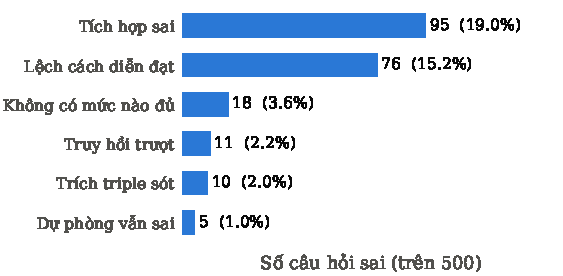
\includegraphics[width=\columnwidth]{figures/fig_errors.pdf}
\caption{Phân loại 215 câu sai theo khâu phát sinh lỗi đầu tiên.}
\label{fig:errors}
\end{figure}

Hình~\ref{fig:errors} xếp 215 câu sai theo khâu phát sinh lỗi đầu tiên. Truy hồi và trích
xuất triple cộng lại chỉ gây ra 21 câu, nên khâu thu thập bằng chứng không phải chỗ nghẽn.
Chỗ nghẽn là giai đoạn tích hợp, nơi mô hình chọn tập triple lõi: riêng khâu này gây ra 95
câu. Thêm 76 câu
nữa đúng nội dung nhưng bị EM cho điểm 0 vì lệch cách diễn đạt (\S\ref{sec:setup}), tức
lỗi của độ đo chứ không phải của phương pháp.

\subsection{Điều kiện dừng thoả quá sớm}
\label{sec:limit-suf}

\begin{table}[t]
\centering\small
\begin{tabular}{lrr}
\toprule
\textbf{Cấu hình} & \textbf{EM} & \textbf{F1} \\
\midrule
Cascade đầy đủ            & 57,00 & 73,05 \\
\midrule
\quad chỉ mức triple      & 57,40 & 72,99 \\
\quad chỉ mức câu         & 60,80 & \textbf{75,38} \\
\quad chỉ mức đoạn        & \textbf{61,20} & 75,16 \\
\quad triple + câu        & 57,00 & 73,03 \\
\quad triple + đoạn       & 56,80 & 72,78 \\
\midrule
\quad $L=1$               & 52,60 & 67,52 \\
\quad $L=2$               & 57,40 & 73,18 \\
\bottomrule
\end{tabular}
\caption{Bóc tách thành phần. Mọi biến thể đều giữ mức dự phòng ở \S\ref{sec:fix}, nên
các dòng so sánh được với nhau nhưng không so trực tiếp được với Table~3 của bài báo gốc.
Hai dòng cuối cho thấy hiệu năng bão hoà từ $L{=}2$.}
\label{tab:ablation}
\end{table}

Cơ chế cascade không mang lại lợi ích nào trong thiết lập của chúng tôi, thậm chí gây hại.
Hai biến thể bỏ hẳn cascade, một luôn đọc mức câu và một luôn đọc mức đoạn, cho kết quả cao
hơn cascade đầy đủ 3,8 và 4,2 điểm EM ($p < 0{,}005$), nên Bảng~\ref{tab:ablation} đi ngược
Table~3 của bài báo gốc.

Cũng chính Bảng~\ref{tab:ablation} chỉ ra nguyên nhân. Biến thể luôn dùng mức triple đạt
57,40, gần như trùng với 57,00 của cascade đầy đủ. Hai cấu hình cho cùng kết quả nghĩa là
cascade hầu như không mở rộng ngữ cảnh, mà dừng ở mức triple đúng 361/500 câu. Lý do nằm ở
tín hiệu nó chờ: $\mathrm{Suf}$ chỉ cho phép mở rộng ngữ cảnh khi mô hình trả về câu từ
chối, mà Gemini 2.5 Flash hiếm khi trả về.

\subsection{Mọi mức ngữ cảnh thừa hưởng thiếu sót của khâu lọc}
\label{sec:limit-empty}

Kiểu lỗi thứ hai là hệ thống từ chối trả lời dù bằng chứng đã nằm trong tay. Cả ba mức đều
dựng từ một tập triple lõi, nên khâu lọc bỏ sót phần nào thì $F$, $S$ và $D$ cùng thiếu đúng
phần đó, và mở rộng ngữ cảnh chỉ là đọc lại cùng một thiếu sót ở dạng dài hơn. Mô hình từ
chối ở cả ba mức, và hệ thống rơi vào nhánh mặc định của Phương trình~\ref{eq:acmg}. Nhánh
này nhận 73 câu, toàn bộ đều sai, nhưng 66 câu trong số đó có recall truy hồi bằng 1,0:
module truy hồi đã lấy về đủ bằng chứng và chính khâu lọc đã loại đi. Nhóm chịu thiệt nặng
nhất là câu hỏi so sánh hai thực thể, 24 trong 51 câu, vì khâu lọc thường chỉ giữ triple về
một trong hai.

\section{Thay điều kiện đủ bằng phép kiểm bằng chứng}
\label{sec:fix}

$\mathrm{Suf}$ dùng câu từ chối làm dấu hiệu cho việc ngữ cảnh đã đủ hay chưa, và dấu hiệu
này sai theo cả hai chiều: mô hình từ chối cả khi bằng chứng đã có sẵn
(\S\ref{sec:limit-empty}), và trả lời cả khi bằng chứng còn thiếu (\S\ref{sec:limit-suf}).
Chúng tôi sửa chiều thứ nhất trước, vì mức cải thiện của hai bản sửa cộng dồn lên nhau.

\paragraph{Mô hình từ chối dù bằng chứng đã có.} Chúng tôi bổ sung một mức cuối không dựng
từ tập lõi: khi không có mức nào trong cascade trả lời được, hệ thống đọc lại toàn bộ đoạn đã
truy hồi. Mức này nâng EM từ 50,80 lên 57,00 và giảm số câu bị từ chối từ 73 xuống 35, với 31
trong 38 câu nó xử lý cho đáp án đúng.

\paragraph{Mô hình trả lời dù bằng chứng còn thiếu.} Ở đây hệ thống chốt ngay mức triple
với một câu trả lời trôi chảy nhưng sai, và đầu ra không có gì báo hiệu. Mô hình không bịa
đáp án: trong 262 câu kiểm được bằng chuỗi, 252 câu có đáp án nằm nguyên trong tập triple
lõi. Nó đọc đúng những triple nhận được, chỉ là tập triple đó chưa đủ.

Tập nào đủ và tập nào chưa thì đo được: mỗi triple đều lưu vết đoạn đã sinh ra nó, nên ánh
xạ provenance $M^D$ (\S\ref{sec:cirag}) cho biết cả tập lõi đến từ bao nhiêu đoạn khác nhau.
Nhóm mà cả tập lõi chỉ đến từ một đoạn đạt 35,7 EM, nhóm đến từ hai đoạn đạt 71,6. Vì mọi câu hỏi ViMQA đều cần bằng chứng từ ít nhất hai đoạn, tập lõi gói trong một đoạn
là chưa đủ về mặt cấu trúc, bất kể mô hình có sẵn lòng trả lời hay không.

Chúng tôi vì vậy thêm một điều kiện trên bằng chứng bên cạnh điều kiện sẵn có trên câu trả
lời:
\begin{equation}
\label{eq:newsuf}
\mathrm{Suf}'(a, F) = \mathrm{Suf}(a) \cdot \mathbf{1}\!\left[\lvert M^D(F) \rvert \ge h\right]
\end{equation}
với $h$ là số tài liệu câu hỏi đòi hỏi. Không thoả thì hệ thống bỏ qua các mức hẹp và đọc
thẳng mức rộng nhất. Phép kiểm chỉ đọc lại thông tin có sẵn nên không tốn thêm lời gọi mô
hình, và $h = 2$ suy từ cấu trúc bộ dữ liệu chứ không dò trên tập đánh giá.

\paragraph{Kết quả.} Với cả hai thay đổi, CIRAG chuyển từ chỗ kém IRCoT sang hơn IRCoT
(Bảng~\ref{tab:main}). Riêng phép kiểm mới đóng góp 3,40 điểm ($p = 0{,}0005$), với 20
câu được sửa đúng so với 3 câu bị làm sai. Khi chúng tôi đổi mô hình nền sang Qwen3-30B-A3B, cải tiến vẫn cùng chiều nhưng nhỏ
hơn và chưa đạt ý nghĩa thống kê (55,40 lên 57,00 EM, $p = 0{,}12$). Đáng chú ý là trên cả
hai mô hình nền, CIRAG sau cải tiến đều hơn IRCoT đúng 1,4 điểm, còn trước thì bằng hoặc kém.

\paragraph{Hạn chế của cải tiến.} Nó không vượt được biến thể luôn đọc mức đoạn ở
Bảng~\ref{tab:ablation}: 60,40 so với 61,20, $p = 0{,}56$.

\section{Loại trừ bốn cách giải thích}
\label{sec:backbone}

Mỗi cách giải thích được kiểm bằng một thí nghiệm chỉ đổi đúng một biến. Phép tái lập ở
\S\ref{sec:results} đã loại cách thứ nhất, lỗi cài đặt. Với cách thứ hai, prompt tiếng Việt
do chúng tôi viết còn prompt tiếng Anh là của nhóm tác giả, nên đây là biến gây nhiễu có
thật. Chúng tôi chạy lại cả 500 câu bằng prompt gốc và thu được 57,40 EM so với 57,00, phân bố mức ngữ cảnh
gần như không đổi.

Cách thứ ba đòi so từng khâu giữa hai bộ dữ liệu trên cùng mô hình nền. Recall truy hồi, tỷ
lệ tích hợp giữ được ít nhất một triple, và tỷ lệ sinh được truy vấn kế tiếp đều lệch dưới
năm điểm.

Cách thứ tư cần một đính chính, vì kết quả đổi dấu tuỳ mốc so sánh. Nếu lấy NativeRAG làm
mốc thì khoảng cách của CIRAG co từ 8,8 xuống 1,8 điểm khi mô hình nền mạnh lên, nhưng NativeRAG
đọc thẳng cả mười đoạn nên hưởng lợi bất thường từ mô hình mạnh, và chỗ co lại phản ánh
NativeRAG khá lên chứ không phải CIRAG kém đi. Còn nếu lấy IRCoT làm mốc thì đổi mô hình nền chỉ dịch
chuyển khoảng cách 0,8 điểm, so với 15,2 điểm do đổi bộ dữ liệu.

\paragraph{Điều còn lại.} Sau khi loại cả bốn, phần chênh lệch duy nhất đạt ý nghĩa thống kê
nằm ở loại câu hỏi: CIRAG hơn IRCoT 4,5 điểm ở nhóm câu đúng/sai ($n = 156$,
$p = 0{,}15$) nhưng kém 4,9 điểm ở nhóm câu mở ($n = 344$, $p = 0{,}031$). Câu mở đòi hỏi tái
tạo nguyên văn một cụm từ, đúng chỗ nén ngữ cảnh thành triple gây thiệt vì triple đã lược bỏ
cách diễn đạt gốc.

\section{Kết luận}
\label{sec:conclusion}

Lợi thế 14 điểm của CIRAG không xuất hiện trên ViMQA, và nguyên nhân nằm ở chính điều kiện
dừng của phương pháp. Điều rút ra được vượt ra ngoài CIRAG: một điều kiện dừng suy từ hành
vi của mô hình chỉ đáng tin chừng nào mô hình còn bộc lộ hành vi đó, mà mô hình nền càng
mạnh thì càng ít bộc lộ. Một điều kiện đặt lên chính bằng chứng không để chỗ cho kiểu lỗi
âm thầm đó.

\section*{Hạn chế}

Kết luận chính dựa trên hai bộ dữ liệu, mà phép tái lập trên 2WikiMQA chỉ chạy 100 câu
hỏi với kho ngữ liệu 770 đoạn, nhỏ hơn hẳn 1.000 câu của bài báo gốc. Thiết lập nhỏ hơn
khiến truy hồi dễ hơn, nên phép tái lập chỉ có giá trị một chiều: nó bác bỏ được nghi ngờ
cài đặt sai, nhưng không chứng minh được bản cài đặt tương đương hoàn toàn.

Việc loại trừ vai trò của mô hình nền dựa trên hai mô hình, đủ để thấy đóng góp của yếu tố
này nhỏ so với yếu tố bộ dữ liệu, nhưng chưa đủ để mô tả quan hệ theo năng lực. Cuối cùng, hai trường hợp EM cho điểm 0 dù đúng (\S\ref{sec:setup}) ảnh
hưởng tới cả ba phương pháp: riêng 99 câu có đáp án tham chiếu dài đã chiếm 89 trong 215
câu sai của CIRAG.

\bibliography{custom}

\end{document}
